\section{Further improvements}
We were able to create a prototype system that met all of the client requirements before the deadline.
If our prototype is chosen for further development there are some obvious next steps that would begin implementation immediately.

\subsection{Frontend aesthetics}
While the current frontend is functional (Figure~\ref{fig:fe}), it is difficult to use and not aesthetically pleasing.
The user experience design is non-existent, and while it fulfills the business logic, it does not function in a way that allows advanced users to capitalize on the structure of the frontend to perform actions more efficiently.

\begin{figure}[tbph]
  \centering
  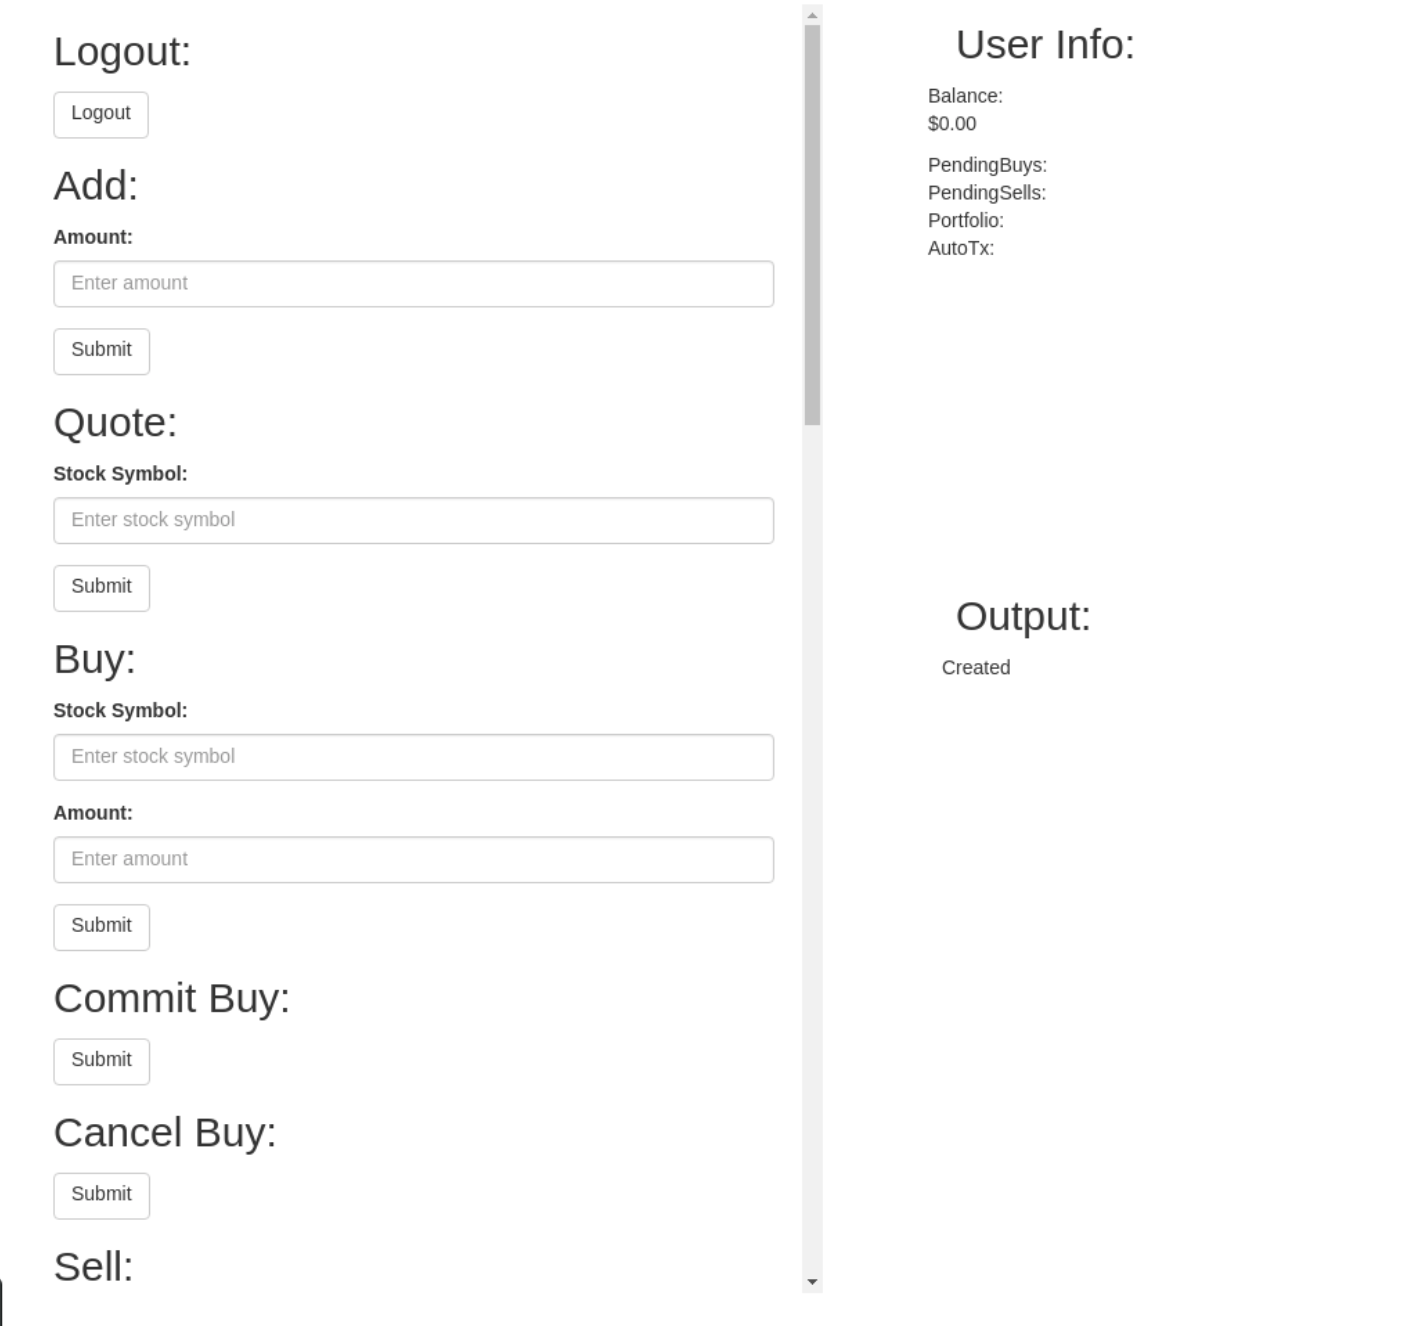
\includegraphics[width=0.7\linewidth]{graphics/fe}
  \caption{Current frontend design}
  \label{fig:fe}
\end{figure}

\subsection{Encryption}
While the websockets are a one-to-one connection between the user, the information is not currently encrypted in any sort of way that would prevent a Man In The Middle (MITM) attack.
In the very near future, we would enjoy performing end-to-end encryption to protect the user's information as it transitions through the websphere.

\subsection{Social media authentication}
While our current authentication system allows much freedom for management on the backend, it is but another “roll your own” authentication system that the user must create an account for.
By adding social media authentication such as Facebook or Google Oauth, we would decrease the barrier of entry for new users to enter the platform.
By doing this we could grow the larger user numbers, and work on the scalability of the system if users were to near tens or hundreds of thousands.
Facebook currently has almost 2 billion users, and allowing these users access to our system in one click is an incredible way to promote user growth.
Additionally the current authentication system stores user information in the browser’s localstorage.
A competent user could modify their localstorage account info to that of another user and gain unauthorized access to their account.
This security hole would be eliminated by the use of social media authentication.

\subsection{Higher TPS}
Additional TPS can be achieved by adding new workers.
A thorough discussion of the limits and methods for scaling is in~\ref{sec:scaling}.

\subsection{Mesos or Kubernetes deploy}
Docker proved to be relatively useful for setup/teardown of RMQ, Redis and other services.
However, any time we wanted to do a VM deploy, we would be forced to manually run each docker instance and set everything up.
Further improvements would include the addition of Apache Mesos or Google Kubernetes for managing Docker deployments.
This would cut down significantly on setup time for full scale runs, as well as allow simple runtime tweaking for different environments such as production or testing.
